\chapter{Theory and Methods}
\section{{Introduction}}\label{intro}
\newline \newline \noindent
In this chapter, the theories and methods used in this Thesis will be the main point of focus. The problem under consideration is the adoption of DERs and the utility death spiral for different policies. In this system, there will be many complex processes going on in the system, like emergence, adaptation, prediction, and state-based responses because of the interactions between different households and the DSO. Therefore, the system under consideration, it will be treated as a complex adaptive system (CAS). Since this type of system requires an appropriate modeling technique to account for all the complexities and details embedded within its structure, agent-based modeling (ABM) is an appropriate modeling technique to do so. Within the ABM, a decision making theory will be required to account for the decision-making patterns of the households in the investment process. Cumulative prospect theory will be implemented to incorporate human behavior in the decision-making process.
\newline \newline \noindent
In the following sections of this chapter, the different theories and methods are to be discussed. First, in section \ref{CAS}, the properties of CAS will be the main point of focus. Subsequently, in section \ref{Prospect}, the decision making theories relevant to this Thesis will be discussed. Since the selected decision making theory (cumulative prospect theory) belongs to behavioral economics, this broader topic of science will be the first point of discussion before elaborating on the specific characteristics and equations related to both prospect theory (PT) and cumulative prospect theory (CPT). In this discussion, a few alternatives to the CPT will also be highlighted, like the expected utility theory (EUT) and the rank-dependent utility theory. These different theories will also be compared to the CPT. In section \ref{Modeling}, the different modeling techniques that can be used to address the problem under consideration will be covered. These techniques include optimization modeling, equilibrium modeling and agent-based modeling (ABM). Each of these modeling techniques has its specific properties, advantages, and drawbacks, which will be discussed and synthesized in this section. In section \ref{approach}, research approach will be elaborated upon in detail in Chapter 4.
\section{Complex Adaptive Systems} \label{CAS}
The notion of what a complex adaptive system (CAS) entails is important in the selection of an appropriate modeling technique. The literature surrounding CAS, however, fails to give a formal definition or overview of what a CAS exactly is. Intuitively, however, the different characteristics of a CAS can be explained. According to \cite{ABM}, an adaptive system is one that, over time, will improve its relation to the environment. This can be any kind of environment: a physical, biological, social, technical or cultural one, just to name a few. Adaptations are not the same as change in response to a stimulus, since a change can be for better or for worse, whereas an adaptation always is for the better. These stimuli are from the environment itself and must also appear in some patterns in the system, either on a constant or a regular basis. Note that an adaptation is not the same as an evolution, since evolution is the aggregate effect (or algorithm) of all adaptations that produce all these improvements, as was examined by Charles Darwin in his "Origin of Species"\cite{Darwin}. Based on the stimuli that the system/environment will produce, therefore, agents in a CAS will gradually adapt their behavior to increase their synergies with the situation presented by the environment. This behavior is often referred to as self-organization. When a system develops over time, through emergent behavior, patterns and structures in the system will arise. These patterns and structures are not predefined in the model, but are a consequence of actions performed by the actors in the system. Self-organization is the result of these adaptive responses of the actors, which will gradually shape the system \cite{ABM}. 
\newline \newline \noindent
A complex system is, to put it bluntly, the opposite of a simple system. This simplicity can be either structural or functional. When simulating systems, however complex the assumptions and models are, there will always be some simplifications or limitations imposed on the system. In ABM, however, it is possible to capture these complexities to a decent level, allowing for the modeling of CAS. 
\newline \newline \noindent
Railsback identified several key characteristics of CAS for modeling the complex dynamic behavior of agents in a system \cite{6CAS}. These will be discussed over the next few points:
\begin{itemize}
    \item \textbf{Emergence}: One of the key elements of CAS is the emergence of system-level properties. Although the emergent behavior of the properties will occur on a system level, it is a consequence of the character traits of agents and individuals. If the emergence of properties follows from simple decision rules, it is possible to predict how different properties will emerge from different sets of decision rules. It is also a good guarantee that the model is general and can be applied to untested situations. The approach to system modeling, in this case, is very different compared to optimization and equilibrium modeling: rather than describing the CAS from a system level, which can require a large number of equations for advanced models, the system is described from an agent/individual level. For more complex models, this often allows for a more straightforward definition of the rules. The emergent response of agents cannot be confused with imposed response of agents. The latter forces agents to make certain decisions or perform certain actions in a specific situation. These imposed responses are often the result of what has been observed in real-world experiments. The validity of the imposed responses is, therefore, limited to the situations that have been observed in the field. For a generally valid model, therefore, the responses must be extended beyond the empirical situations available. Ideally, the model should be designed in a mechanistic rather than an empirical manner. The decision should also be formalized in a mechanistic way (i.e., the agent should make decisions or perform actions based on a minimal/maximal value of a certain parameter, surpassing a certain threshold value, etc.). In doing so, the empirical limitations of a model are removed. If the emergent response of a mechanistic model resembles the imposed response from the empirical findings, it is safe to assume that this emergent behavior is generally applicable to different situations. Therefore, the important traits of the agents are necessary knowledge to design a model.
    \item \textbf{Adaptation}: Together with emergence, adaptation is one of the core elements of CAS. As has been discussed in previous paragraphs, adaptation refers to the ability of agents to improve their fitness in their environment through behavioral changes. Depending on the complexity of the model, a system can show elementary or very advanced adaptive behavior. Although adaptation stems from biological evolution, which is an adaptive process that took many centuries, this behavior in CAS can occur in different spatial and temporal scales. As a function of these spatial and temporal scales, the relevant characteristics that must be adaptive can be identified: short-term adaptations must be a function of a relevant short-term event (like the adaptation of animals becoming more aggressive when they suddenly feel threatened) while long-term adaptations should be a function of the relevant long-term events (to stay with the animal example, the physiology of animals will adapt as the weather patterns in their environment gradually evolve).
    \item \textbf{Fitness and strategy}: The definition of fitness in the context of CAS must be clearly defined in the scope of the problem at hand. Fitness in a model is the state agents are seeking to obtain by optimizing their synergies with the environment. This seeking process will happen through a series of adaptive actions. The concept of fitness is important to define rules that will allow the agents to adapt their behavior. If fitness for the different agents is not defined, the adaptive actions cannot be clearly defined either. This fitness strategy can also be a function of the state of the agents and a function of time.
    \item \textbf{State-based responses}: Agents in the CAS will, since they will have adaptive character traits, respond to certain stimuli that the environment exposes them to. This response, however, is not a static response, but rather a dynamic response depending on the state or situation the agents finds himself in. Animals living in ecosystem, for instance, will hunt and move about depending on their fitness. In the case of investment decision making, people with large savings and capital reserves will be more likely to invest in new, uncertain technologies, whereas people with limited savings and capital reserves will be less prone to invest in such technologies.
    \item \textbf{Prediction}: Since the agents in a CAS show intelligent behavior, these agents will be able to predict or anticipate the occurrence and outcome of certain events. This anticipation and prediction is a result of a learning process from past experience throughout the evolution of the system. This predictive ability appears in the most simple CAS (bacterial models) as well as very advanced CAS (like population behavior models). Holland identified two different kinds of prediction: tacit and overt \cite{CAS}. Tacit prediction happens when actions are performed based on assumptions that are implicitly present in the model since they are considered commonly accepted knowledge (for example, underlying physical models in a system). Overt predictions happen on a more explicit basis since the assumption are explicit in the model and action will be taken accordingly. Decisions will be made by forecasting different alternatives and considering the consequences of these alternatives, only to choose the most promising alternative. Being able to distinguish the different alternatives and computing their possible outcomes is key in understanding the adaptive behavior of agents. 
    \item \textbf{Computer simulations}: For the vast majority of all cases, the simulation of agent behavior in CAS relies on computer simulations. Since the development of a CAS and its implementation in computer code almost always goes hand in hand, the formulation and implementation of CAS models must be considered jointly. In this perspective, an important part of the relation between the conceptual model and computer implementation is the user interface of the model. To understand a CAS and its adaptive/emergent traits, studying the input-output evolution of a model is very important, so the way in which a model will provide output to the user is very important. Although the representation of output variables increases the computational requirements of a model, it is a vital part of a computer program to understand and improve its functioning. If the output of a model is simply taken for granted and the model itself is treated like a black box, a recipe for disaster from a model validation point of view is presenting itself. In addition to having a good user interface, the model must be well documented in detail, since a small attribute of a model can easily render it erroneous. By fully documenting a model, it becomes easy to decompose and reproduce by other researchers. The ODD protocol can serve as a good framework to perform this model description. Finally, there must be sufficient quality control of the computer code and results that the model produces to ensure the validity of the model.
\end{itemize}
% justify the selection of ABM as a modelling technique
A visualisation of a CAS can be found in Figure \ref{Figure:CASS}. Here, the emergent behavior of self-organising sets of agents can be seen. The feedback loops causing the adaptive behavior between the environment and agents are also represented in the Figure.
\newline 
\begin{figure}[h!]
\centering
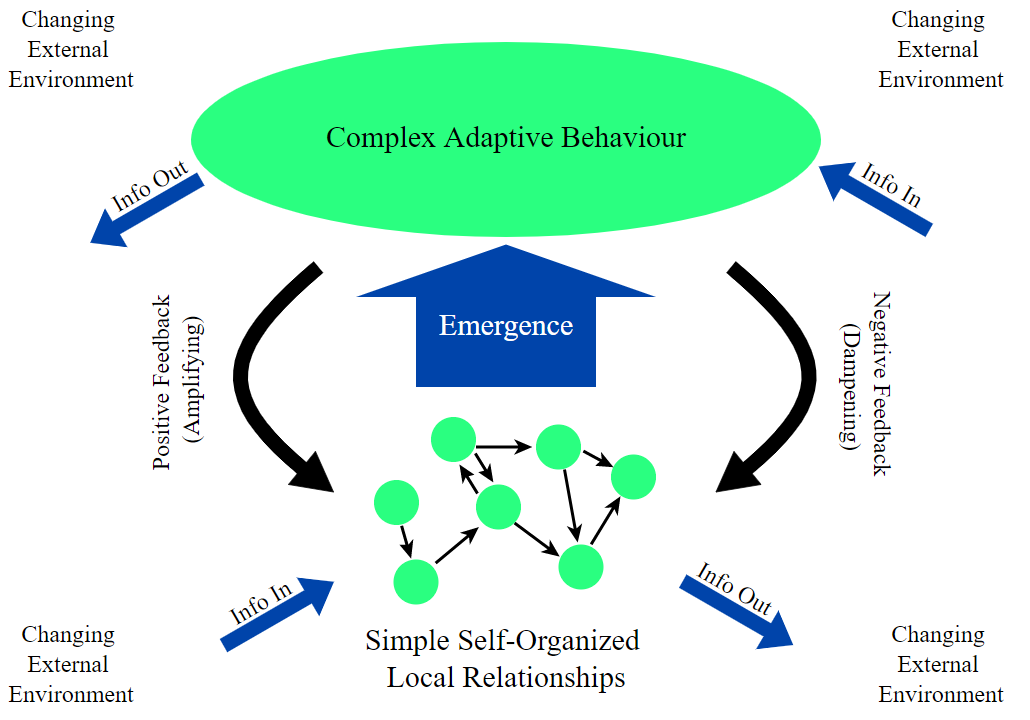
\includegraphics[width=10cm]{Complex_adaptive_system.png}
\caption[Conceptual example CAS]{Conceptual example CAS \cite{CAsexample}}
\label{Figure:CASS}
\end{figure}
\newline \noindent
Since these system characteristics imply a great deal of dynamics, like emergence and adaptive behavior, an appropriate modeling technique will be required to simulate these dynamics. As will be discussed in section \ref{Modeling}, agent-based modeling is the preferred technique over other techniques like optimization and equilibrium modeling.
 
\section{{Decision-making theories}} \label{Prospect}
\subsection{\large{Introduction}} 
Since the model in this Thesis deals with the simulation of decision making on a household level, an appropriate decision making theory must be selected to account for sub-optimal, irrational decision making traits. As will become clear over the course of this section, behavioral finance or economics are a branch of science that can help account for sub-optimal decision making on a household/individuals level. From the different theories in behavioral finance, cumulative prospect theory (CPT) will emerge as the preferred candidate for the simulation of decision making. 
\newline
\newline
Over the course of this section, the scene will first be set by broadly discussing behavioural finance and economics. Subsequently, the specifics of prospect theory will be discussed. In doing so, a brief history and a summary of the theory will be the main focus. Finally, prospect theory will be compared to other theories of choices under risk that have been developed over the last few decades in parallel with it. 
\subsection{\large{Behavioral economics}}
As the name suggests, behavioral economics deals with the economic implications of human behavior. In doing so, this starts from observations of actual human behavior, which behavioral economists attempt to formalize into a theory. Empirical data in this field will, therefore, constantly challenge a certain theory. Many theories in behavioral economics will subsequently only be as good as the experiments it describes. This makes it challenging for the theories to be operational, which is still is one of the major challenges in this branch of science. Although having been in development for many decades, behavioral economics has been gaining lots of popularity in recent years through recognition of the highest academic level for renowned scientists like Daniel Kahneman \& Vernon L. Smith in 2002 \cite{NobelKahne}, Eugene F. Fama, Lars Peter Hansen \& Robert J. Shiller in 2013 \cite{Nobelshiller} and Richard H. Thaler in 2017 \cite{Nobelthaler}. This recognition has strengthened the case for behavioral finance and economics, which strongly opposed itself to the classical economics theories of rational choices.
\newline \newline \noindent
In classical economic theory, which can be traced back to the principles first postulated by Adam Smith, many ideal assumptions prevail about decision making in economics \cite{adamsmith}. In a world existing under these assumptions, people make decisions based on fully informed calculations whose results they interpret rationally. These choices will also align with the best self-interest of the decision-making agent. This agent will often be referred to as the "homo economics", since the agent is assumed to be an economically rational human being, putting economic considerations in decision making before any other consideration. This approach to economic thinking was later incorporated in the theory that is often referred to as rational choice theory. This rational choice theory (RCT hereafter) serves as an umbrella term for theories in neoclassical economics, where the outcomes of certain actions can in some way be construed as rational \cite{RCT}. This "ensemble" of theories, often referred to as neoclassical economics, relies on three major assumptions:
\begin{itemize}
  \item Individuals have selfish preferences
  \item Individuals maximize their utility
  \item Individuals act independently based on full information
\end{itemize}
\noindent
The most "simple" version of neoclassical economics/RCT assumes that all individuals are fully informed about all decisions alternatives, the probabilities of their outcomes, their consequences and assumes no cognitive limitations for the agent in the processing of all this information. These assumptions are very strict and demanding and can, therefore, hardly be implemented for real-life experiments. Herbert Simon, therefore, introduced the concepts of bounded rationality in 1957 \cite{boundedrat}. This concept relaxes the assumptions of full rationality. Under bounded rationality, the agent/decision maker recognizes that gathering information is an energy and time demanding process, thereby limiting the amount of information that will be gathered and processed for decisions making. Whereas full rationality is the process of "maximizing" someone's situation, bounded rationality is the process of 'satisficing' a certain situation. 
\newline \newline \noindent
In its attempts to reshape economics as a natural science through rationality assumptions and terms such as the "homo economicus", the first economic theories on decision making imposed many ideal assumptions on the behavior of economic agents, creating a very artificial representation of certain models. Through his theory of bounded rationality, Herbert Simon put a limit to these assumptions by saying that rationality is constrained due to limited time to process all information available and limited tractability of the decision problem at hand. This already is the first step in the direction that humans or other decision makers will inevitably make suboptimal choices, away from the economically rational theory developed by neoclassical economists. By the end of the 1960s, as cognitive psychology became a more established and commonly accepted branch of psychology \cite{cognitive}, Kahneman and Tversky used this new development in science to lay the conceptual foundations of prospect theory, which will be discussed in the next section.
\subsection{\large{Prospect theory}} \label{ProspectTheory}
As discussed in the previous subsection, prospect theory (PT) is the result of many different stages in the transition from rational, neoclassical economics assuming that the "homo economicus" will always make economically optimal decisions, to the rationally bounded, cognitive agent that will make sub-optimal decisions that are satisfying, rather than optimal, to him. In this section, the different aspects of prospect theory will be highlighted and discussed. The development of prospect theory arose through lab experiments obtained by Kahneman and Tversky that diverged from the decision making theory that was widely accepted at the time, being the Expected utility theory (EUT). The authors, therefore, postulated a different version of decision making, which will be the main point of attention over the course of the next few paragraphs.
\newline \newline \noindent
When choosing among uncertain scenarios, an agent is choosing from a set of prospects or gambles \cite{prospect1}. A prospect is nothing more than an overview of different outcomes a certain asset evolution have, while taking into account the probability of all these different outcomes. Mathematically, this prospect can be represented as:
 \begin{equation}
     (x_1,p_1; x_2,p_2;...;x_n,p_n)
 \end{equation}
 Where $p_1$ is the likelihood that this contract of outcomes will yield the result $x_1$, $p_2$ the likelihood that the contract of outcomes will yield the result $x_2$, etc.. Note that that this set of probabilities is subject to the constraint:
 \begin{equation}
     p_1 + p_2 + ... + p_n = 1 
 \end{equation}
The assumptions EUT makes around these prospects (see section \ref{EUT}) had already been severely challenged by previous work. This can be divided into a few different parts. First of all, there was significant criticism in what is referred to as the \textit{certainty effect}. If this effect is manifesting itself, people overweight outcomes that are considered certain, relative to outcomes which are perceived as probable. A good case for this certainty effect is given in \cite{Allais}. What also arose from these test is that in a case where winning is possible but not probable (i.e. there are gains to be made but the likelihood of receiving them is small), most people choose the prospect that offer the larger gain. A second aspect where EUT failed, according to Kahneman and Tversky, is the incorporation of negative prospects. This effect, referred to as the \textit{reflection effect} by the authors of PT \cite{prospect1}, states that the preference between positive and negative prospects are the mirror image of each other. This brings with itself an important factor of PT, more specifically that risk aversion in the positive domain (i.e. when facing gains) is accompagnied by risk seeking in the negative domain (i.e. when facing losses). Parts of this theory had already been suggested by previous research, only to be reconfirmed by Kahneman and Tversky \cite{Marko} \cite{Williams}. Besides the two aforementioned criticisms, which are the main criticism PT had on EUT, there are many more mentioned in \cite{prospect1}, but a discussion of all these points are out of the scope of this research. It is worth noting that over the course of their academic career, Kahneman and Tversky provided an initial prospect value theory in \cite{prospect1} in 1979 and provided an update in 1992, called the cumulative prospect theory (CPT) \cite{prospect2}. Over the course of the 1980s, prospect theory came under increasing criticism by other theories, like the rank dependent theory (see section \ref{EUT}). In the classical theory, the utility of an uncertain prospect is the sum of the utilities of the outcomes, each weighted by its probabilities \cite{prospect1}. The new CPT, however, provides a few updates. Based on the finding of the rank-dependent utility theory, the probability function now is of the cumulative kind. Since CPT is the updated version of the initial PT, this is the version of the theory that will be used in this Thesis. Nevertheless, a quick overview of the original theory and its subsequent improvement will be given in the next few paragraphs
\newline \newline \noindent
The original PT divided the decision making process into two different stages: the editing phase and evaluation phase. This was done to avoid any violation of first-order stochastic dominance in the results. In the editing phase, all the options are laid out and reformulated to simplify the evaluation or organisation of the decision making. Different outcomes will be classified as either gains or losses compared to a certain reference point, which usually is the current asset position of the decision maker\footnote{A generally accepted definition of this reference point hasn't been formulated yet, which is one of the main reasons why PT is not operationalizable}. All prospects will also be simplified and segregated into riskless and risky prospects. This editing will be based on heuristics, which means that the decisions will be motivated by past experiences of the decision making agent. 
\newline \newline \noindent
Following the editing phase, the evaluation phase will kick off and the decision maker will value each of the prospects and choose the one with the highest value. This selection will be done according to the computation of the value $V(x)$:
\begin{equation}
    V(x) = \sum_{i=1}^{n} \pi(p_i)*v(x_i)
\end{equation}
\noindent
With $\pi(p_i)$ the decision weight and $v(x_i)$ the subjective value of the outcome to the agent. Note that at the time of the first publication of PT, there was no formal definition of how to compute these components. Together with the criticism that came once published, particularly from Quiggin's rank-dependent utility theory (see section \ref{EUT}), all these items were updated and formalised in the CPT \cite{prospect2}.
\newline \newline \noindent
The value function $v(x)$ in CPT can be described using the following set of functions:
\[   \left\{
\begin{array}{ll}
      x^\alpha & x \geq 0 \\
       -\lambda(-x)^\beta & x < 0 \\
\end{array} 
\right. \]
\newline 
Where \textit{x} is the prospect variable. As in PT, this variable will be the difference between a certain outcome and the reference level of the prospect variable. This reference level can be defined in several ways, like a constant value or a reference value given a certain riskless asset. The exponents $\alpha$ and $\beta$, representing the risk aversion, are both equal to 0.88, as was determined by Kahneman and Tversky after having performed and extensive amount of tests. The final parameter of the value function equation, $\lambda$, is the loss aversion coefficient. Through their experiments, Kahneman and Tversky set this value of this parameter at 2.25. These values, however, have never been obtained in replications of the experiments done by the authors of CPT. The values obtained by Kahneman and Tversky, however, were measured separately, which would allow for them to be duplicated in this Thesis. Nevertheless, these values (the loss aversion in particular) are quite high compared to other more recent experiments. These differences in loss and risk aversion as well as a selection of an appropriate value will be discussed in Chapter 4. A graphical representation of a possible value function can be found in Figure
\ref{Figure:value}.   
\newline 
\begin{figure}[h!]
\centering
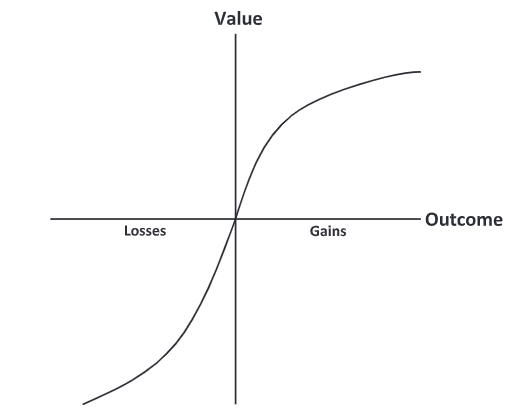
\includegraphics[width=7cm]{ValueFunction.PNG}
\caption[Representation of hypothetical value function]{Representation of hypothetical value function, based on \cite{prospect2}}
\label{Figure:value}
\end{figure}
\newline \noindent
Another aspect that needs further discussion in cumulative prospect theory is the so called probability weighting function. Based on their initial findings and later those of the rank-dependent utility theory, Kahneman and Tversky realized that people will not objectively perceive the probabilities of certain outcomes. This has been researched in many domains of psychology, beyond the applications of prospect theory \cite{Weighting}. In this work, the authors postulate that, as is the case in prospect theory, decision makers will not treat probabilities linearly. As can be seen in Figure \ref{Figure:weight}, the weighting function of a linear probability curve shows has an inverse-S-shaped evolution. 
\newline 
\begin{figure}[h!]
\centering
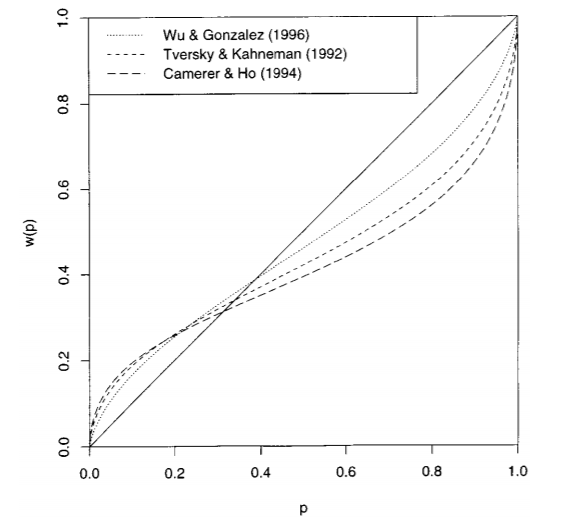
\includegraphics[width=8cm]{weighting-functions.png}
\caption[Representation of distorted weighting probability function]{Representation of distorted weighting probability function \cite{Weighting}}
\label{Figure:weight}
\end{figure}    
\newline
The evolution of this curve has been supported in several studies \cite{prospect2} \cite{Weighting2} \cite{Weighting3}. The probability weighting curve is concave for low probabilities (close to 0) and convex for higher probabilities (closer to 1). Intuitively, the evolution of this weighting function can be explained as the fact that people become less sensitive to changes in probability as this probability moves further away from the reference point. These reference point are the probabilities where a certain outcome 'is gonna happen for sure' or 'not going to happen at all', so 0 and 1. The evolution of the weighting function, therefore, will be more extreme when moving towards the reference point than when it moves towards the middle of the scale (probability of 0.4-0.6). Kahneman and Tversky referred to this effect as \textit{Diminishing Sensitivity}. The equation that satisfies this weighting function is:
\begin{equation}
    w^{+}(p) = \frac{p^{\gamma}}{(p^{\gamma} + (1-p)^{\gamma})^{1/\gamma}}
    \label{weight1}
\end{equation}
For positive prospects (i.e. when $x \geq 0$) and 
\begin{equation}
    w^{-}(p) = \frac{p^{\delta}}{(p^{\delta} + (1-p)^{\delta})^{1/\delta}}
    \label{weight2}
\end{equation}
\newline \newline \noindent
For negative prospects (i.e. when $x < 0$). The exponents $\gamma$ and $\delta$ have both been determined through extensive tests by Kahneman and Tversky. The value of $\gamma$ was found to be 0.61 and that of $\delta$ to be 0.69.
\newline \newline \noindent
With all the items of CPT known, a comparison with other behavioral economic theories can be done to determine if prospect theory is the more promising theory to model human behavior in investment decisions under risk. Nevertheless, two alternative decision making theories to prospect theory will be discussed, being expected utility theory (EUT) and rank dependent utility theory.
\subsection{\large{Related theories}}
As mentioned in section \ref{Prospect}, prospect theory is a continuation of different previously established behavioral economics models. In this section, therefore, these different theories will be highlighted. The most related are expected utility theory (EUT) and rank dependent utility theory.
\subsubsection{Expected utility theory} \label{EUT}
Like prospect theory, EUT is a theory to model decision making under risk. Rather than looking at the overall dollar value of a certain decision, EUT will consider the subjective value of a set of choices whose outcome is uncertain. Contrary to PT or CPT, the computation of the utility is very straightforward. Given a set of possible outcomes:
\begin{equation}
    (x_1,p_1;x_2,p_2;...;x_n,p_n)
\end{equation}
Then the expected utility can be calculated using the formula:
\begin{equation}
        E[u(x)] = \sum_{i=1}^{n}    p_i*u(x_i)
\end{equation}
According to EUT, agents will select the maximal utility of a set of possible choices. This computation, straightforward and easy to implement as it may seem, does make a few assumptions that make the theory unreliable and incomplete. The first one is the assumption that probabilities are perceived on a linear basis, which has been disproven by rank dependent utility theory, which will be discussed in the next subsection. In addition, as discussed in section \ref{Prospect}, the EUT fails to make good estimations of the certainty and reflection effect, estimations that were improved by PT. 
\newline \newline 
Despite being developed and postulated over two centuries before prospect theory (the foundations of EUT were laid by cousins Daniel and Nicolas Bernouilli in the so-called St-Peterburg Paradox in the first half of the 18th century \cite{Bernoulli}) and having been a widely accepted decision making model for a long time, recent efforts in behavioral economics have made the concepts proposed in EUT obsolete. This has already been proven in the literature \cite{EUTvsPT}. In this research, EUT and PT are compared as decision making models under risk in financial markets. The application of PT in this work is the so-called smooth prospect theory (SPT). The result from this work, where the authors simulated the behavior of agents populating an artificial market, were much more "realistically"  when using SPT compared to EUT. This already is a first indication that PT is the preferred candidate.
\subsubsection{Rank dependent utility theory}
This theory, developed as a response to the classical prospect theory by Kahneman and Tversky, is a generalised expected utility theory. The new ideas developed in this model were subsequently incorporated by Kahneman and Tversky in their cumulative prospect theory \cite{prospect2}. What makes rank dependent utility theory different from the general utility theory or the initial version of prospect theory, is the idea to introduce a cumulative probability distribution function of the outcome probabilities. This is contrary to using the individual probabilities to different outcomes \cite{rankdependent}. One of the main criticisms on PT that rank dependent utility theory tries to solve is the way the so-called first-order stochastic dominance\footnote{In statistics, a set \textit{F} first-order stochastically dominates a set G if a decision maker weakly prefers \textit{F} over \textit{G} for any weakly increasing utility function} was bypassed by Kahneman and Tversky. Aware of this problem, they introduced the editing phase into their PT \cite{prospect1}. This, however, had additional issues, like violations in transivity\footnote{A relationship \textit{R} over a set of variable {a,b,c} is said to be transitive if whenever \textit{R} relates to a and b and b and c, it also does so to a and c}.
\newline \newline \noindent
The rank-dependent model presented by Quiggin surpassed these issues by introducing transformations to the cumulative probability distribution function, rather than doing so to the probabilities of the outcomes. What Quiggin introduced, was the idea that outcomes with a very low likelihood of occuring will have a disproportionately perceived probability, whereas the probability of other, less extreme outcomes will be perceived normally. Since the innovations of the rank-dependent utility theory were later incorporated into the CPT, the latter theory can be concluded to be the most complete theory in behavioral economics for the modeling of decision making, which is the reason why it is the one that will be used for the remainder of this Thesis. 
\newline \newline \noindent
An overview of the different decision making theories can be found in table \ref{tab:overview1}.
\begin{table}[h!]
    \centering
    \begin{tabular}{||c|c|c|c||}
    \hline 
        \textbf{Theory}  & Flexibility & Complexity & Validity \\
    \hline \hline
         \textit{Expected utility} & Medium & Low & Low \\
    \hline
        \textit{Rank Dependent}  &  Medium & Medium & Medium\\
    \hline 
        \textit{Prospect}  & High & High & Medium\\
    \hline 
        \textit{Cumulative prospect}  & High & Medium & High\\
    \hline 
    \end{tabular}
    \caption{Overview decision making theories}
    \label{tab:overview1}
\end{table}
\subsection{Prospect theory in literature} \label{prospectliterature}
In the previous sections, the different aspects of behavioral economics and finance have first been discussed, followed by a description of the theories involved (prospect theory, expected utility theory and rank dependent utility theory). From this discussion, cumulative prospect theory (CPT) turns out to be the most suitable candidate to model investment decisions under risk. Since this Thesis focuses on investments in power generation and storage assets, it may be interesting to determine whether there has been related research. In doing so, it is important to consider that the research in this Thesis is on a household/prosumer level.  
%\newline \newline \noindent
%There has been research into the consumption-investment behavior of a household in more than one period \cite{Consumption}. In this work, the consumption and investment patterns of a household are analysed using prospect theory. The main purpose of the research is to determine how assets are being allocated, between the more risky ones and riskless ones, compared to the consumption of the household. 
%\newline \newline \noindent
%Prospect theory has also been applied in financial markets, investments and portfolio management\cite{portfoliochoice, portfoliochoicestat, portfoliochoicean}. In both works, cumulative prospect theory (CPT) is used for the optimal portfolio selection with one risk-free asset and one risky asset. This is done in a multi-period setting. In doing so, portfolio constraints are taken into account. In \cite{portfoliochoicestat}, the portfolio returns are static, whereas a stochastic process is imposed on them in \cite{portfoliochoice}. Through numerical simulations, all the different parameters are subsequently tested. In \cite{portfoliochoicean}, this test is done in an analytical manner. In some papers, the focus is rather on multiple assets rather than investments over multiple periods \cite{multistock}. In this work, prospect theory is used to model the investments in a single-period setting with one riskless bond and multiple stocks. From these works in financial markets, authors were able to spot a few trends. As the risk aversion of the agents increased, the proportion of wealth invested in risky assets as a function the entire portfolio increased in parallel. Moreover, the popularity of risky assets decreased as the returns of the assets decreased and/or the volatility of the assets increased. Something the authors of \cite{portfoliochoice} also observed was that the effect of changing risk aversion on the investment decisions in the different portfolio assets decreased over time.
%\newline \newline \noindent
%Besides the previously mentioned fields, prospect theory has also been used in different fields, like the modeling of the investments in spectrum for wireless communication \cite{spectrum}. In this research, the investment problem is defined as a two-stage investment to model the optimal investment strategy under the uncertainty of which actions to do on the spectrum market. In the case of this work, however, the application of prospect leads to a non-convex optimization problem, which brought an additional level of difficulty to the model. Contrary to classical prospect theory, however, the operator is both risk averse and loss averse. 
\newline \newline \noindent
Prospect theory has been used in energy research to model the behaviour of agents in domains like energy trading and storage investments \cite{Stackelbergprospect,Storageprospect,consumercentric,loadshift,reactive}. In \cite{Stackelbergprospect}, the interaction between a group of smart grid prosumers on the one hand and a power company on the other hand is studied. Here, the power company will act as a single leader, with multiple followers (this is also called a Stackelberg game). Prospect theory is used in the valuation of the utility of certain gains and losses for the prosumer. In addition, a comparison is made with game theory. In \cite{Storageprospect}, the interaction and exchange of energy of several distributed energy storage units. Prospect theory is used as an alternative to game theory, to make the decision less objective and rational. Since behavior of the operator of the storage unit will deviate from the optimal schedule, it is possible that some undesirable situations present themselves, like undesirable grid loads and revenues. This will cause the central power company to rethink their pricing scheme and the prosumers to change their charging and discharging habits. In \cite{consumercentric}, prospect theory is proposed as a decision-making framework to help understand how risk and uncertainty are perceived by smart grid consumers and how it will shape their investment decisions. In \cite{loadshift}, the same logic of irrational, non-optimal decision making is applied to load shifting in the context of demand-side management (DSM). Most of the work concerning DSM assumes agents will be objective and fully rational agents, which is an oversimplification this work tries to rephrase. In \cite{reactive}, finally, the authors attempt to apply the same logic to the valuation customers will perform of the compensation value for reactive power compensation. Contrary to most studies who let the agent optimize the objective value of the reactive power compensation value, this work lets agents optimize the subjective value of the reactive power compensation.  In the aforementioned works, the authors acknowledge that PT can increase the ability of simulating decision-making of actors in the energy market. They also claim the potential of PT is underdeveloped and will become a key modeling technique in the design and analysis of consumer-centric energy systems like smart grids. Considering this support for CPT in energy-related research, using this theory in the setting of this Thesis is permitted. 
\section{{Modeling Methods}} \label{Modeling}
\subsection{\large{Introduction}}
In this section, the different modeling techniques will be discussed that can be used for the simulation of investment decision in the electricity sector. First, the equation based models (optimization and equilibrium modeling) will be discussed, followed by the modeling technique that will be used in this dissertation, being agent-based modeling (ABM). In discussing the different modeling techniques, the focus will mainly be on their validity in modeling a human process that investing (usually)\footnote{Nowadays, many so-called quantitative hedge funds use computer models to invest in securities without any human intervention, sometimes with amazing results} is, especially in the context of this Thesis. This includes discussing their advantages as well as their shortcomings. 
\subsection{\large{Optimization modeling}}
The most traditional kind of modeling technique for decision making is optimization modeling \cite{optimization}. The basic premises for this technique is finding the best possible solution from a set of alternatives. Usually, there will be a finite amount of possible solutions to the problem, which is often referred to as the feasible region. Even if the model is formulated as a continuous problem, a computer solver will discretize the model, making the set of solutions limited. The size of the feasible region is limited by so called 'constraints', which are conditions imposed on the problem that limit the values that certain variables in the equations can have. Often, these constraints will be of a physical nature, like mass balances, temperature constraints or process efficiencies, to name a few.
\newline \newline \noindent
An optimization problem can mathematically be represented as an objective function that needs to be either maximized or minimized (like a cost function):
\begin{equation}
    {min/max}_{x} \; f(x)
\end{equation}
Where the feasible region is constrained by a set of equality constraints:
\begin{equation}
    h(x) = 0
\end{equation}
and inequality constraints:
\begin{equation}
    g(x) \leq 0
\end{equation}
Taking into account these boundary conditions, the optimal solution to this problem, which gives the maximal/minimum value of the objective function and corresponding parameter values, can be obtained. Often, the objective function and constraints will be a function of many process variables. The final optimization model can come in many different forms, like a linear problem (LP), non-linear problem (NLP), mixed-integer linear problem (MILP) and mixed-integer non-linear problem (MINLP), to name a few. To obtain the optimal solution of this set of objective function and (in)equality constraints, a multitude of solution methodologies are available, like the Newton-Rhapson method and steepest descent method for NLPs, just to name a few.
\newline \newline \noindent
Optimization is used in many different engineering processes, like chemical processes, thermal networks and electronic filter design, to name a few. In electricity investment decision models, this method has been considerably used in the past \cite{Optimization1,Optimization2,Optimization3}. This has gradually been substituted by other models, which shall be discussed in the next subsections. Since optimization modeling offers a rigid framework for the model formulation and follows a rigorous path to obtain a solution, it is a very accessible way to analyse a system and obtain an optimal solution. Once  the variables involved in a system are known, the objective that needs to optimized and the limitations of the system, the solution lies within reach. This makes it such a good candidate for the modeling of physical/chemical processes. For processes that involve human behavior, however, there are a few issues with this modeling technique. First of all, the optimization of a system implies that an actor has access to all information concerning the system, which rarely is the case in an investment decision process. Moreover, optimization modeling implies that the agent/decision maker will make choices on a rational basis. Both these assumptions, unfortunately, are oversimplifications of the complex process that investment decision making is. More complex modeling techniques like equilibrium modeling and agent-based modeling, which will be discussed later in this chapter, therefore, make it possible to capture these process complexities.  
%It must be noted, however, that although optimization modeling will not be the prevailing decision making technique in this Thesis, it will serve as a method to solve a "sub-problem" of the overall model. To calculate the optimal cost savings of a given PV-battery configuration, an optimization problem with certain boundary conditions will be formulated and used in the model. The objective function, constraints and solutions to this problem will be discussed in chapter 4, when the model development will be the main point of discussion. 
\subsection{\large{Equilibrium modeling}}
Whereas optimization modeling will strive to find the optimal solution of a certain set of equations, equilibrium modeling is a more specific technique to determine the equilibrium between different actors. This equilibrium can be competitive, cooperative or a leader-follower equilibrium, like a Stackelberg game. Equilibrium modeling, therefore, is more focused on economic optimization, whereas optimization modeling can be applied to any kind of process. In practice, therefore, different actors will perform an optimization of a certain system and make a decision from their point of view. Based on these optimality conditions, the equilibrium can be determined \cite{Poncelet}. This will be the point where the gains of all agents combined will be maximal. A common example is the equilibrium between the consumer and producer surplus in a supply-demand curve. The total surplus will be maximized by the different agents (consumers and producers) performing a personal optimization and choosing prices and quantities accordingly. A schematic overview of an equilibrium model can be found in Figure \ref{Figure:equi}. 
\begin{figure}[h!]
\centering
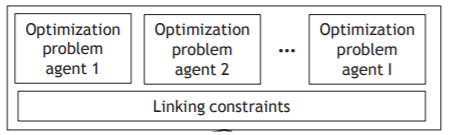
\includegraphics[width=10cm]{Equilibrium.PNG}
\caption[Graphical representation of an equilibrium model]{Graphical representation of an equilibrium model (source: \cite{Poncelet})}
\label{Figure:equi}
\end{figure}
\noindent
Besides the fact that this modeling technique will 'decentralise' the decision making process whereas optimization modeling has a centralised starting point, this modeling technique can incorporate market inefficiencies. Contrary to optimization modeling, this modeling technique can relax some assumptions regarding efficient markets, perfect information and rational decision making. It is, however, still an equation based modeling technique that will solve a set of processes towards an equilibrium, which makes it difficult to capture the dynamics of complex adaptive systems, which real-world systems often are. Since the focus in this Thesis is on the emergence of PV-battery adoption through economic utility and interaction between agents, equilibrium modeling may not be the best technique to model this adaptive process. Agent-based modeling, which will be discussed in the next subsection, will be able to capture the properties of CAS. 
\subsection{\large{Agent-based modeling}} \label{AgentBased}
The previously discussed modeling methods are able to solve a certain process (represented by a set of equations) and find its optimal configuration. This solution, however, is a 'static' solution. For a given set of equations, optimization and equilibrium modeling will find a unique solution to this problem. This methodology is useful in systems that strive towards a certain static state of optimal equilibrium, like heat transfer processes or chemical reactions. The modeling of CAS, where emergent, adaptive and self-organizing behavior of the agents, to name few, have to be accounted for, requires a more comprehensive modeling technique. This technique must be able to surpass the equation-based description of a certain process. ABM will be able to do that, by subjecting the agents in the CAS to a set of rules they must abide, in an attempt to create a more realistic simulation of a dynamic  phenomenon.
\newline \newline \noindent
Whereas advanced optimization and equilibrium models require large sets of equations to describe a system, agent based models will add an additional level of complexity to the description and simulation of these processes by moving away from a top-down system description (as is done in optimization and to a certain extent in equilibrium modeling). On the contrary, ABM's approach will be the exact opposite, by describing the system bottom-up in the form of behavior rules. This added level of complexity is introduced into the modeling approach to improve the descriptive capabilities of the model. The trade-off is the added level op complexity and computation time for ABMs. An ABM will consist of agents, who will dynamically interact with each other in their environment. Throughout the simulation of the agents' behavior in the environment, agent interaction will give rise to emergent properties on a system level. Note how this property is aligned with the emergent property of a CAS. ABM has a few advantages compared to the previously discussed techniques. Since the construction and simulation of the model are a bottom-up process, agent characteristic can be simulated, monitored and analysed more efficiently. When considering how the emergent properties of a system manifest themselves, as is the case in this Thesis, ABMs can be a very useful tool to visualise this emergence. Another advantage of ABM is the possibility to study the path dependence of a certain process. The 'trajectory' of the model over the course of its simulation period can be observed, providing valuable insights in the model dynamics of a system. Since optimization or equilibrium models will converge to a certain system or process equilibrium, this path dependence cannot be observed as easily. With any advantage also comes a disadvantage, which in the case of ABM is modularity. Since this modeling technique can be applied in a wide range of applications to describe and simulate the behavior of CAS, ABM will not have a standard framework like optimization modeling to formulate and solve the model. The developer of an ABM, therefore, must pay close attention to the characteristics and important parameters of the system to formalise these into a well functioning model. A good understanding of the underlying principles of a model are necessary to ensure a good development of an ABM.
\newline \newline \noindent
This modeling technique, therefore, will serve as the technique to simulate the investment decisions in DERs on a household level. An overview of the different modeling techniques can be found in table \ref{tab:overview2}.
\begin{table}[h!]
    \centering
    \begin{tabular}{||c|c|c|c|c||}
    \hline 
        \textbf{Modeling technique} & Framework & Flexibility & Complexity & Validity \\
    \hline \hline
         \textit{Optimization modeling} & Standard & Medium & Medium & Low \\
    \hline
        \textit{Equilibrium modeling} & Standard &  High & Medium & Medium\\
    \hline 
        \textit{Agent-based modeling} & Modular & High & High & High\\
    \hline 
    \end{tabular}
    \caption{Overview modeling techniques}
    \label{tab:overview2}
\end{table}
Contrary to the optimization and equilibrium modeling techniques, which have a standard framework to formulate the model and generate a solution, the agent-based modeling method requires a more modular approach. As is the case in this Thesis, optimization models and other theories (like CPT or EUT) will be used as building blocks of the overall ABM (see Chapter 4). By combining all these building blocks with respect to agent properties and system interaction, a comprehensive model can be developed. This can make the model description more realistic, but it also requires a thorough understanding of the system under consideration.
\section{Research approach} \label{approach}
The system description in this Thesis relies on CAS theory. The underlying theory can help identify these elements, as well as the relationships among those elements that need to be considered for the analysis and description of a CAS. One of those elements (i.e., adaptation) is described by using the concepts of prospect theory. The most recent version of prospect theory, being the CPT, will be used to that end. 
\newline \newline \noindent
The concept of adaption is further formalized by using prospect theory. Since adaptation in the model is a change in the means of electricity production for the household, the adaptation will translate itself in the adoption of DERs of PV-battery systems. The simulation of this adoption process will be accounted for using CPT, which will subsequently become part of the ABM. The other components of the CAS, being emergence and state-based responses, will be directly embedded in the ABM. A conceptual overview of the model approach can be seen in Figure \ref{Figure:approach}.
\newline 
\begin{figure}[h!]
\centering
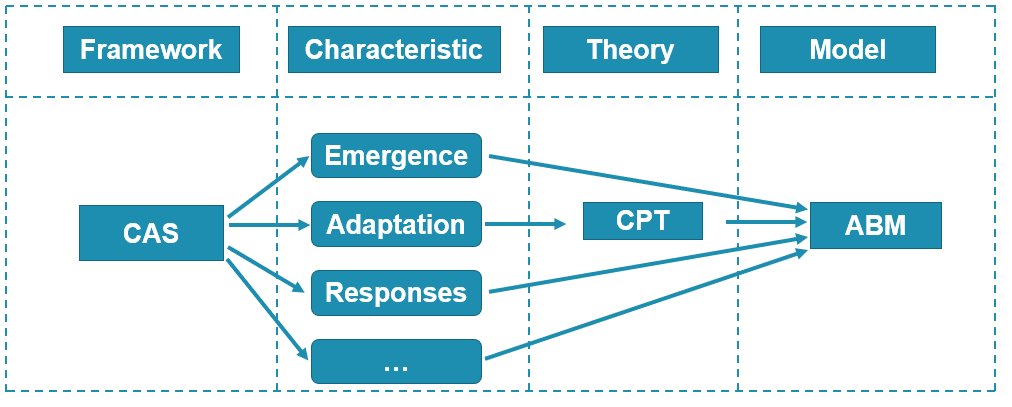
\includegraphics[width=10cm]{approach.PNG}
\caption{Graphical representation of modeling approach}
\label{Figure:approach}
\end{figure}
\newline \noindent
A detailed description of the how these concepts were formalized into an ABM will be the main point of focus in Chapter 4.